%% 2/18/2016
%%%%%%%%%%%%%%%%%%%%%%%%%%%%%%%%%%%%%%%%%%%%%%%%%%%%%%%%%%%%%%%%%%%%%%%%%%%%
% AGUJournalSample.tex: this sample file is for articles formatted with LaTeX
%
% This sample file includes commands and instructions
% given in the order necessary to produce a final output that will
% satisfy AGU requirements.
%
% PLEASE DO NOT USE YOUR OWN MACROS
% DO NOT USE \newcommand, \renewcommand, or \def.
%
% FOR FIGURES, DO NOT USE \psfrag or \subfigure.
% DO NOT USE \psfrag or \subfigure commands.
%
%%%%%%%%%%%%%%%%%%%%%%%%%%%%%%%%%%%%%%%%%%%%%%%%%%%%%%%%%%%%%%%%%%%%%%%%%%%%
%
% All questions should be e-mailed to latex@agu.org.
%
%%%%%%%%%%%%%%%%%%%%%%%%%%%%%%%%%%%%%%%%%%%%%%%%%%%%%%%%%%%%%%%%%%%%%%%%%%%%
%
% Step 1: Set the \documentclass
%
% There are two options for article format:
%
% 1) PLEASE USE THE DRAFT OPTION TO SUBMIT YOUR PAPERS.
% The draft option produces double spaced output.
% 
% 2) numberline will give you line numbers.

% Tip:
%  To add line numbers to lines in equations:
%  \begin{linenomath*}
%  \begin{equation}
%  \end{equation}
%  \end{linenomath*}


%% To submit your paper:
\documentclass[linenumbers,draft]{agujournal}

% Now, type in the journal name: \journalname{<Journal Name>}
% ie,
\journalname{Earth and Space Science}

%% Choose from this list of Journals:
%
% JGR-Atmospheres
% JGR-Biogeosciences
% JGR-Earth Surface
% JGR-Oceans
% JGR-Planets
% JGR-Solid Earth
% JGR-Space Physics
% Global Biochemical Cycles
% Geophysical Research Letters
% Paleoceanography
% Radio Science
% Reviews of Geophysics
% Tectonics
% Space Weather
% Water Resource Research
% Geochemistry, Geophysics, Geosystems
% Journal of Advances in Modeling Earth Systems (JAMES)
% Earth's Future
% Earth and Space Science


%% ------------------------------------------------------------------------ %%
%
%  ENTER Title Page commands:
%
%% ------------------------------------------------------------------------ %%

% (List authors by first name or initial followed by last name and
% separated by commas. Use \affil{} to number affiliations, and
% \thanks{} for author notes.  
% Additional author notes should be indicated with \thanks{} (for
% example, for current addresses). 

% Example: \authors{A. B. Author\affil{1}\thanks{Current address, Antartica}, B. C. Author\affil{2,3}, and D. E.
% Author\affil{3,4}\thanks{Also funded by Monsanto.}}

% (include name and email addresses of the corresponding author.  More
% than one corresponding author is allowed in this LaTeX file and for
% publication; but only one corresponding author is allowed in our
% editorial system.)  

%% Corresponding Author:
% Corresponding author mailing address and e-mail address:

% Example: \correspondingauthor{First and Last Name}{email@address.edu}

% Authors are individuals who have significantly contributed to the
% research and preparation of the article. Group authors are allowed, if
% each author in the group is separately identified in an appendix.)

% \affiliation{1}{First Affiliation}
% \affiliation{2}{Second Affiliation}
% \affiliation{3}{Third Affiliation}
% \affiliation{4}{Fourth Affiliation}

%% Keypoints, final entry on title page.
% Example: 
% \begin{keypoints}
% \item	List up to three key points (at least one is required)
% \item	Key Points summarize the main points and conclusions of the article
% \item	Each must be 100 characters or less with no special
% characters or punctuation 
% \end{keypoints}

%% \begin{abstract} begins second page 

%%%%%%%%%%%%%%%%%%%%%%%%%%%%%%%%%%%%%%%%%%%%%%%%%%%%%%%%%%%%%%%%%%%%%
% Track Changes:
% To add words, \added{<word added>}
% To delete words, \deleted{<word deleted>}
% To replace words, \replace{<word to be replaced>}{<replacement word>}
% To explain why change was made: \explain{<explanation>}

% At the end of the document, use \listofchanges, which will list the
% changes and the page and line number where the change was made.

% When final version, \listofchanges will not produce anything,
% \added{} word will be printed, \deleted{} will take away the word,
% \replaced{}{} will print only the 2nd argument.
% \explain will not print anything.

% Optional argument:
% You can also add additional information to be printed with the list
% of changes, to indicate the initials of the person changing the text,
% and the time and/or date of the change, or any other comment by using
% the optional [] argument:
% \added[AH, 3:30pm, Feb 18, 2016]{added term}
% will yield 
% [AH, 3:30pm, Feb 18, 2016] added term on page...
%%%%%%%%%%%%%%%%%%%%%%%%%%%%%%%%%%%%%%%%%%%%%%%%%%%%%%%%%%%%%%%%%%%%%

\begin{document}

%% ------------------------------------------------------------------------ %%
%
%  TITLE
%
%% ------------------------------------------------------------------------ %%


\title{FITS format for planetary surfaces: definitions,
applications and best practices.}

%% ------------------------------------------------------------------------ %%
%
%  AUTHORS AND AFFILIATIONS
%
%% ------------------------------------------------------------------------ %%

 \authors{C. Marmo\affil{1},
 T. M. Hare\affil{2},
 S. Erard\affil{3},
 M. Minin\affil{4},
 F.-X. Pineau\affil{5},
 A. Zinzi\affil{6,7},
 B. Cecconi\affil{3},
 A. P. Rossi\affil{4}}

\affiliation{1}{GEOPS, Univ. Paris-Sud, CNRS, Univ. Paris-Saclay,
Orsay, France}
\affiliation{2}{U. S. Geological Survey, Astrogeology Science Center,
Flagstaff, AZ, USA}
\affiliation{3}{LESIA, Observatoire de Paris, PSL Research University,
CNRS, Sorbonne Universit\'es, UPMC Univ. Paris 06, Univ. Paris Diderot,
Sorbonne Paris Cit\'e, Meudon, France}
\affiliation{4}{Jacobs University, Bremen, Germany}
\affiliation{5}{Observatoire astronomique de Strasbourg, Universit\'e de Strasbourg, CNRS, UMR 7550, 11 rue de l'Universit\'e, 67000, Strasbourg, France}
\affiliation{6}{ASI Science Data Center, c/o ASI, Via del Politecnico snc, 00133, Rome, Italy}
\affiliation{7}{INAF-OAR, Via Frascati n. 33, 00078, Monte Porzio Catone (RM), Italy}

%% Corresponding Author
%(include name and email addresses of the corresponding author.  More
%than one corresponding author is allowed in this Word file and for
%publication; but only one corresponding author is allowed in our
%editorial system.)  

\correspondingauthor{C. Marmo}{chiara.marmo@u-psud.fr}

%  List up to three key points (at least one is required)
%  Key Points summarize the main points and conclusions of the article
%  Each must be 100 characters or less with no special characters or punctuation 

\begin{keypoints}
\item Inter-operable data formats 
\item Planetary data standards
\item Data processing and visualization
\end{keypoints}

%% ------------------------------------------------------------------------ %%
%
%  ABSTRACT
%
%% ------------------------------------------------------------------------ %%

\begin{abstract}
Planetary science encompasses a broad number of research fields and
brings together several research communities (geologists, astronomers,
physicists, geochemists, etc.). Planetary missions produce an impressively growing 
amount of diverse data requiring an evolution from a mostly manual-based visual 
analysis to a more automated and quantitative analysis.
Interoperability, openness of data formats, and shared processing techniques are
becoming a necessity to efficiently extract scientific information from the data and 
to guarantee the reproducibility of the scientific results.
Unfortunately, the technologies and data formats used by researchers for
planetary surface studies and the field of astronomy 
diverged as these related, but almost completely isolated domains evolved.  
% * <thare@usgs.gov> 2018-02-13T00:44:29.292Z:
% 
% > Unfortunately, the technologies 
% > and data formats used by researchers for planetary surface studies and the field of astronomy 
% > diverged as these related, but almost completely isolated domains evolved.  
% 
% Is this too strong a statement?
% 
% ^.
In this paper we will will describe how a small addition to the Flexible Image Transport System (FITS) 
standard, widely used in the astronomy investigations,  will allow FITS to be more easily used in planetary
surface investigations , we will  show  how FITS metadata can easily be transformed in the PDS4 metadata
archival model, and lastly provide example implementations.
More than imposing a formal data model, a FITS description for planetary data aims
to simplify sharing data across the planetary and astronomy domains and promoting
interoperability from data acquisition to final visualization.
\end{abstract}

%% ------------------------------------------------------------------------ %%
%
%  TEXT
%
%% ------------------------------------------------------------------------ %%

\section{Introduction}
\label{sec:intro}
Planetary science brings together several research communities
(geologists, astronomers, physicists, geochemists, etc.),
and planetary missions produce a growing amount of heterogeneous data.
To efficiently extract scientific information from those data, they must
be made integrable, thus interoperable.
Openness of data format and processing techniques is becoming a necessity,
to guarantee the reproducibility of the results obtained from those data.

This paper proposes to use Flexible Image Transport
System\footnote{https://fits.gsfc.nasa.gov/}
(FITS) format \citep{fitsorig,fitsver3} in planetary surface investigations,
and describes how FITS metadata can easily be inserted in the
PDS4\footnote{https://pds.nasa.gov/tools/standards-reference.shtml}
metadata distribution model.
FITS is one of the standard formats implemented in the Virtual
Observatory\footnote{http://www.ivoa.net/astronomers/using\_the\_vo.html}
(VO), therefore making obvious its connection to the Planetary Virtual
Observatory initiative and the planetary Table Access Protocol (EPN-TAP)
\citep{ERARDepntap}.
FITS format is open and flexible, largely implemented in open and efficient
processing tools.
Those reasons make FITS format appropriate to automatically handle large amounts of raster data.
The goal of this approach is to make easier data mining and reprocessing
in planetary surface investigations, promoting general software based on those
standards.
The option to use FITS within the planetary surface domain could potentially
homogenize methods from acquisition, to visualization, while
giving chances to optimize data processing.

This paper is organized as follows:
\begin{enumerate}
\item{a brief description of FITS format;}
\item{a proposition for planetary surface metadata description in FITS;}
\item{dictionaries between FITS, PDS metadata description and EPN-TAP2.0
parameters;}
\item{some examples of planetary dataset in FITS;}
\item{current developments for making FITS more usable to handle data
of planetary surfaces.}
\end{enumerate}

\section{FITS Format in Planetary Surface Investigation}
\label{sec:fitspss}

\subsection{FITS Format}
FITS is an open digital standard, defined for data acquisition and archiving
in astronomical observatories in the late 70's, and it is used for
spatial telescope data.
The International Astronomical Union approved FITS as the standard format
for astronomical data\footnote{https://fits.gsfc.nasa.gov/iaufwg/history/IAU\_1982\_resolution\_c1.html}. 
Therefore, FITS is one of the standard formats implemented in the Virtual
Observatory\footnote{http://www.ivoa.net/astronomers/using\_the\_vo.html}
(VO).
Finally, FITS data storage is compatible with the Planetary Data System (PDS)
archiving specifications and supported by a large number of open libraries
and software tools.

FITS is already able to propose standard formatting for some data products
quite common by now in planetary surface investigations.
In particular, the Multi-Extension FITS (MEF) schema proposes an easy way
to store inhomogeneous digital information (reflectance, calibration data,
vector, table data, etc.) in the same file, each with corresponding metadata,
as well as multi-detector imagery (e.g. from HiRISE \citep{hirise})
or hyperspectral cubes with geometry information (e.g. from CRISM
\citep{crism} or OMEGA \citep{omega} instruments).
FITS has been already chosen to distribute data from, e.g.,
Hayabusa AMICA and NIRS cameras\footnote{http://darts.isas.jaxa.jp/planet/project/hayabusa/index.html},
all Akatsuki cameras\footnote{http://darts.isas.jaxa.jp/planet/project/akatsuki/index.html}
(except the Lightning and Airglow Camera),
and the Dawn Framing Camera\footnote{https://sbn.psi.edu/pds/archive/dawn.html} data.
In addition, many PDS3 datasets in the Small Bodies Node include FITS files.
To be efficiently used in planetary surface investigations, FITS metadata must
be extended in order to take into account the size of the reference body.
Planetary body shapes and orientations are well defined and standardized by
the IAU Working Group on Cartographic Coordinates and Rotational Elements
(WGCCRE).
This group reports triennially \citep{wgccre} on the preferred rotation rate,
spin axis, prime meridian, and reference surface for planets and satellites
ensuring that cartographic endeavors are effectively comparable.
In the framework of the VESPA\footnote{http://europlanet-vespa.eu/}
\citep{vespapss} workpackage of the EuroplanetRI2020\footnote{http://www.europlanet-2020-ri.eu/}
project an extension to FITS metadata (GeoFITS) has been
proposed\footnote{https://voparis-confluence.obspm.fr/display/VES/GeoFITS:+Planetary+Data+FITS+format+and+metadata+convention},
taking into account the WGCCRE recommendations.

\subsection{Planetary Surface Proposed Convention}
\label{ssec:geofits}
When willing to use FITS format for planetary surfaces the issue of rigorous
geographical representation must be addressed.
For their mapping and analysis needs planetary researchers commonly use
Geographical Information Systems (GIS).
In general, GIS applications excel in data interoperability even
though some have historically been anchored to Earth's spatial description.
Several of them are based on the Geospatial Data Abstraction
Library\footnote{http://www.gdal.org} (GDAL), released by the Open Source
Geospatial Foundation.
GDAL is essentially a format translation library written in C++ for geospatial raster
and vector data and, fortunately, it also offer basic support for FITS format.

FITS World Coordinate System
representation\footnote{http://fits.gsfc.nasa.gov/fits\_wcs.html} is the standard
way to describe spatial dependencies in FITS metadata.
WCS simplifies the spatial coordinate description with respect to historical
terrestrial references.
F
or instance, there is no need for oblique projection definitions
\citep{calagreisenI,Snyder1987} as projection parameters
(projection center or reference point)
describe the difference between, e.g., the Mercator and
Oblique Mercator or Simple Cylindrical and
Equirectangular map projections.
This simplification is effective when a spherical local approximation
is applied on planetary imagery.
This is particularly the case with growing image resolutions and
increasing computing capabilities: spherical projections with a local
radius definition are easier to reproject from one system to another, than
from or to a global spheroidal datum.
As an example, the HiRISE team has chosen to distribute HiRISE projected
products using Equirectangular projection (CAR) on a local surface, approximated
by the sphere with radius equivalent to the local Mars spheroid radius.

In addition, WCS resolves the ambiguity between east-handed and west-handed
longitude systems, as the pixel conversion in world coordinates is set by an
oriented matrix.
If needed, FITS does offer the possibility to fully describe the projected
coordinate system using several alternative WCS definitions (meters, degrees,
East and West longitude, etc.)\citep{greisencalaII}.

Table \ref{table:proj} summarizes the FITS projection codes and their
corresponding PDS4 projection names (see table A.1. in \citet{calagreisenI}
for details).

\begin{table}
\label{table:proj}
\caption{Projection names and codes already available in FITS suitable for
planetary applications: the corresponding PDS4 terminology is
provided.}
\centering
\begin{tabular}{l l l}
\hline
FITS Name$^{a}$ & FITS code$^{a}$ & PDS name$^{b}$ \\ 
\hline
Zenithal Equidistant & ARC & Azimuthal Equidistant \\
Zenithal Perspective & AZP & General Vertical Near-sided Projection \\
Plate Carre & CAR & Equirectangular, Miller Cylindrical \\
Equidistant Conic & COD & Equidistant Conic \\
Conic Equal-Area & COE & Albers Conical Equal Area \\ 
Conic Ortomorphic & COO & Lambert Conformal Conic\\
Mercator & MER & Mercator, Oblique Mercator, Transverse Mercator \\
Polyconic & PCO & Polyconic \\
Sanson-Flamsteed & SFL & Sinusoidal \\
Ortographic & SIN & Orthographic \\
Stereographic & STG & Stereographic, Polar Stereographic \\
Gnomonic & TAN & Gnomonic \\
Zenithal Equal-Area & ZEA & Lambert Azimuthal Equal Area \\
\hline
\multicolumn{3}{l}{$^{a}$From \citet{calagreisenI}} \\
\multicolumn{3}{l}{$^{b}$From the PDS4 Data Dictionary\footnote{https://pds.jpl.nasa.gov/pds4/doc/dd/current/PDS4\_PDS\_DD\_1900.pdf}. We cannot find correspondences in the WCS scheme for PDS4 Robinson,} \\
\multicolumn{3}{l}{Van Den Grinten and Space Oblique Mercator.}
\end{tabular}
\end{table}

Once reprojected in one of the standard projections listed in Table \ref{table:proj}
Planetary images or maps can be described using the WCS scheme
\citep{greisencalaII,calagreisenI}.
In WCS context pixels are first translated in an intermediate pixel coordinate system
via linear transformations, then mapped on the grid specified by the \texttt{CTYPE}
keyword, containing the projection code and the coordinate system.
The coordinate system must be defined with respect to a specific inertial reference frame.

Multiple coordinate system descriptions are allowed in the same header: this is a valuable
property for planetary surface imagery, as angular ('deg') and linear ('m') description of
the surface are often needed at the same time.
Further below 3D keyword will be proposed for FITS metadata, in order to standardize
the conversion between angular and linear coordinates: alternate description will still
be important in our framework as standard libraries (e.g.
wcslib\footnote{http://www.atnf.csiro.au/people/mcalabre/WCS/wcslib/} or
astropy\footnote{http://www.astropy.org/} \citet{astropy}) and some FITS visualization
software (e.g. ds9\footnote{http://ds9.si.edu/}) already implement them, making linear
coordinate tracking more efficient.  

\subsubsection{FITS WCS keywords and their recommended use in planetary surface context}
\label{sssec:wcskeys}
In this section WCS FITS keywords are inserted in the planetary surface context.
When possible, corresponding PDS4 and EPN-TAP definitions are added for archiving
standardization purposes.
\begin{enumerate}
\item{RADESYS.
Name of the inertial reference frame with respect to which the coordinate
system is defined (defaulted to \texttt{'ICRS'})}
\item{EQUINOX.
The value field contains the equinox in years for the celestial
coordinate system in which positions are expressed (defaulted to \texttt{'J2000'})}
\item{WCSAXES.
Number of axes in the WCS description.
The value of WCSAXES may exceed the number of raster pixel axes.}
\item{WCSNAME.
Name of world coordinate descriptions (e.g. body-fixed rotating -ocentric -ographic,
non-rotating, inertial).
EPN-TAP provides a \texttt{spatial\_coordinate\_description} parameter.}
\item{CRPIXn.
Location of a reference point along axis $n$, in units of the axis index.
The reference point value do not need to lie within the actual data array.}
\item{CTYPEn.
Name of the coordinate represented by axis $n$, in “4–3” form: the first four characters
specify the coordinate type, the fifth character is a '-' and the
remaining three characters specify an algorithm code for computing the world coordinate
value (\ref{table:proj}).
For angular coordinates \citet{calagreisenI} provides the form xLN xLG or yzLN yzLG, where x or yz
are listed in Table \ref{table:ctype}.
For linear coordinates we propose a similar scheme: xPX as Projected X, xPY as Projected Y,
or yzPX and yzPY.
Alternative representation of WCS are already possible in FITS, to describe images in degrees
and in meters \citep{greisencalaII}.
The name of the alternative axis will be specified using the alternative CNAMEn keyword.}
\item{CRVALn.
Value of the coordinate specified by the CTYPEn keyword at the reference point CRPIXn.}
\item{CDi\_j.
The $ij$ linear transformation matrix (rotation, skewness, scaling) defining the intermediate
world coordinates.}
\item{PCi\_j.
The $ij$ linear transformation matrix (rotation, skewness) defining the intermediate pixel
coordinates (to be used with CDELT keywords).}
\item{CDELTn.
The coordinate increment along axis $n$ (scaling component of the linear transformation
matrix PCi\_j).
In PDS4 they correspond to the \textit{pixel\_resolution\_x} and \texttt{pixel\_resolution\_y}
attributes.
In EPN-TAP they are connected to the \texttt{spatial\_resolution} parameter.}
\item{CUNITn.
Units of the coordinate system , not mandatory, defaulted to deg for angular coordinates
and to meters (m) for linear ones.}
\item{CNAMEn.
The description of a particular coordinate for an axis in a particular WCS (up to 68
characters), while the WCSNAMEa keyword names the particular WCS as a whole.
Its default value will be blank.}
\end{enumerate}

\begin{table}
\label{table:ctype}
\caption{Codes to be used in CTYPE FITS keyword in order to identify the planetary body.
Codes for planets are assumed in \citet{calagreisenI}. We propose to add codes for classes of targets,
more or less corresponding to PDS4 Target type attribute and to EPN-TAP target\_class parameter.}
\centering
\begin{tabular}{l l}
\hline
Body & CTYPE$^{a}$ \\ 
\hline
Moon & SE \\
Venus & VE \\
Mars & MA \\
Jupiter & JU \\
Saturn & SA \\
Uranus & UR \\
Neptune & NE \\
Satellites (other than the Moon) & ST \\
Asteroids & AS \\
Dwarf Planets & DW \\
Comets & CO \\
\hline
\multicolumn{2}{l}{$^{a}$From \citet{calagreisenI}}
\end{tabular}
\end{table}

Nevertheless, WCS does not record information about the body shape and
orientation, and reference surface.

\begin{sidewaystable}
\label{table:newkeys}
\caption{Proposed keywords are related to 3D surface shape,
not available in astronomical celestial standards.}
\centering
\begin{tabular}{l l l l}
\hline
Keyword & Type & Status & Definition  \\
\hline
WGCCRECS & string & reserved & Value field contains a string referring to the WGCCRE report \\
& & & or document defining the coordinate system describing the data. (DOI)    \\
A\_RADIUS$^{a}$ & real & mandatory & Value field contains the semi-major axis of the ellipsoid that \\
& & & defines the approximate shape of a target body used in projection. \\
& & & 'A' is usually in the equatorial plane. Always in meters.  \\
B\_RADIUS$^{a}$ & real & mandatory & Value field contains the value of the intermediate axis of \\
& & & the ellipsoid that defines the approximate shape of a target body used in projection. \\
& & & 'B' is usually in the equatorial plane. Always in meters.   \\
C\_RADIUS$^{a}$ & real & mandatory & Value field contains the value of the semi-minor axis of the \\
& & & ellipsoid that defines the approximate shape of a target body used in projection. \\
& & & 'C' is normal to the plane defined by 'A' and 'B'. Always in meters. \\
OGCCODE	& string & reserved, optional & Value field contains a string describing the standard OGC code \\
& & & (if any) from \citet{hare2006} corresponding to the shape and projection used in the image. \\
& & & This keyword will assure compatibility with standard GIS softwares. \\
\hline
\multicolumn{4}{l}{$^{a}$Note that IAU Working Group defines a mean radius for each Solar System body. When this Mean Radius is used in projection definition,} \\
\multicolumn{4}{l}{  the three keywords A\_RADIUS, B\_RADIUS,C\_RADIUS, must be set to the same value of the defined Mean Radius.} \\
\end{tabular}
\end{sidewaystable}

\subsubsection{Correspondence Between Reserved FITS Keywords and PDS4 Standard Reference}
\label{sssec:stdfitspds4}
The correspondence between mandatory and reserved FITS keywords (as defined in
the last version of the FITS standard document\footnote{https://fits.gsfc.nasa.gov/standard40/fits\_standard40aa.pdf})
and PDS4 attributes, is described here.
\begin{enumerate}
\item{\texttt{BITPIX}.
It specifies the number of bits that represent a data value in
the associated data array.
PDS4 uses the attribute \texttt{data\_type}: corresponding 
values depend on the associated object class.}

\item{\texttt{NAXIS}.
It contains a non-negative integer representing the number of axes in
the associated data array.
A value of zero signifies that no data follow the header.
PDS4 uses \texttt{axes}, always defined as a non-negative integer.}

\item{\texttt{NAXISn}.
It contains a non-negative integer representing the number of
elements along axis \texttt{n} of a data array.
The \texttt{elements} attribute of the PDS4 \texttt{Axis\_Array} class provides
the count of the number of elements along an array.}

\item{\texttt{BUNIT}.
It contains a string, describing the physical units in which the quantities
in the array are expressed.
The units of all FITS header keyword values should conform with the recommendations
in the IAU Style Manual\footnote{https://www.iau.org/publications/proceedings\_rules/units/}.
For angular measurements given as floating point values, degrees are the recommended
units (with the units, if specified, given as 'deg').
PDS4 specifies in the class Element (of a vector, array, or any other class
containing Elements), a \texttt{unit\_id}} (unit abbreviation) and a \texttt{unit}
(unit long name).

\item{\texttt{BSCALE}.
It contains a floating point number representing the coefficient of the linear term
in the scaling equation $physical\_value = BZERO + BSCALE \times array\_value$,
the ratio of physical value to array value at zero offset.
For all classes containing Elements, PDS4 defines a \texttt{scaling\_factor}
attribute.
Both FITS and PDS4 default this value to $1$.}

\item{\texttt{BZERO}.
It contains a floating point number representing the constant term in the
scaling equation $physical\_value = BZERO + BSCALE \times array\_value$
For all classes containing Elements, PDS4 defines a \texttt{value\_offset}
attribute. Both FITS and PDS4 default this value to $0$.}

\item{\texttt{BLANK}.
This keyword must be used only with integer data.
It contains an integer that specifies the value that is used to
represent pixels that have an undefined physical value.
On floating point data the IEEE NaN must be used to represent undefined values.  
\texttt{PDS4 Special\_Constants?}}

\item{\texttt{DATAMAX}.
It always contains a floating-point number, giving the maximum valid physical value represented
by the array, excluding any IEEE special values.
PDS4 defines a \texttt{valid\_maximum} attribute in the \texttt{Special Constants} class
having this same meaning.}

\item{\texttt{DATAMIN}.
It always contains a floating-point number, giving the minimum valid physical value represented
by the array, excluding any IEEE special values.
PDS4 defines a \texttt{valid\_minimum} attribute in the \texttt{Special Constants} class
having this same meaning.}

\item{\texttt{DATE}.
It contains the date on which the file was created, provided as ISO 8601
string.
PDS4 provides a \texttt{creation\_date\_time} attribute defining date
and time of product creation.}

\item{\texttt{DATE-OBS}.
It contains the date of the observation, provided as ISO 8601
string. The value shall be assumed to refer to the start of the observation,
unless another interpretation is clearly explained in the comment field.
It is assumed to be expressed in UTC but other systems are accepted as long as they
are specified in the ISO string\footnote{See table 30 in the Standard FITS document https://fits.gsfc.nasa.gov/standard40/fits\_standard40aa.pdf}. 
PDS4 provides a \texttt{Time\_Coordinates} class with attributes
\textit{start\_date\_time} and \texttt{stop\_date\_time} providing start and
stop date and time appropriate to the product being labeled, always in UTC.
The \texttt{time\_min} and \texttt{time\_max} fields are mandatory in the EPN-TAP scheme,
they must always be formatted in UTC as a ISO string (planned in EPN-TAP v2.1).}

\item{\texttt{INSTRUME}.
It contains a character string identifying the instrument used to acquire the data.
PDS4 provides an \texttt{Instrument} class which attribute \texttt{Name} ideally 
corresponds to this FITS keyword.
EPN-TAP provides with an \texttt{instrument\_name} parameter.}

\item{\texttt{TELESCOP}.
It contains a character string identifying the telescope used to acquire the data.
The PDS4 \texttt{Instrument\_Host} class provides the description of the physical object
mounting the instrument. Its \texttt{Name} attribute should correspond to the FITS keyword.
PDS4 also provides for the definition of a \texttt{Telescope} class, in case of
ground-based observations.
In the EPN-TAP scheme this is introduced by the \texttt{instrument\_host\_name}
parameter\footnote{https://naif.jpl.nasa.gov/pub/naif/toolkit\_docs/FORTRAN/req/naif\_ids.html\#Spacecraft}.}

\item{\texttt{OBJECT}.
It contains a character string giving a name for the observed
object\footnote{https://naif.jpl.nasa.gov/pub/naif/toolkit\_docs/FORTRAN/req/naif\_ids.html\#Planets\%20and\%20Satellites}.
The PDS4 \texttt{Target} class contains the \texttt{name} attribute corresponding to this
FITS keyword.
EPN-TAP standard also provides with a \texttt{target\_name} parameter.
Notice that PDS4 and EPN-TAP also ask for a \texttt{target\_type} attribute, which must be
specified from an enumerated list.}

\item{\texttt{ORIGIN}.
It contains string identifying the organization or institution responsible for
creating the FITS file.}

%
%\item{\texttt{AUTHOR}}

\item{\texttt{REFERENC}.
It contains a character string citing the bibliographic reference where the
data are first described.
It is recommended that either the Astrophysics Data System bibliographic
databases\footnote{http://adswww.harvard.edu/}
bibliographic identifier or the Digital Object Identifier\footnote{http://doi.org}
be used.
PDS4 \texttt{External\_Reference} class and EPN-TAP \texttt{bib\_reference} have
exactly the same meaning and use than the FITS keyword.}

\end{enumerate}

\subsection{Examples and Best Practices}

\subsubsection{Visualization of Global and Projected Maps}
High level products are meant to be used for visual inspection or GIS analysis.
They are distributed as projected rasters, often in GeoTIFF\footnote{http://geotiff.osgeo.org/}
format, as GeoTIFF make them GIS ready.
Given some new keywords introduced in FITS and WCS definitions adapted to planetary surface, FITS
and GeoTIFF are completely interchangeable.
As an example we have downloaded some global maps from USGS
Astropedia\footnote{https://astrogeology.usgs.gov/search} and converted them in FITS.
We used ds9 to display the FITS image and were able to visualize coordinates in meters
as in QGIS, a popular open source GIS software, but also in planetary latitude and longitude
thanks to the alternate coordinate
description (see figure \ref{fig:ds9qgis}, left side).
\begin{figure}[ht!]
\centerline{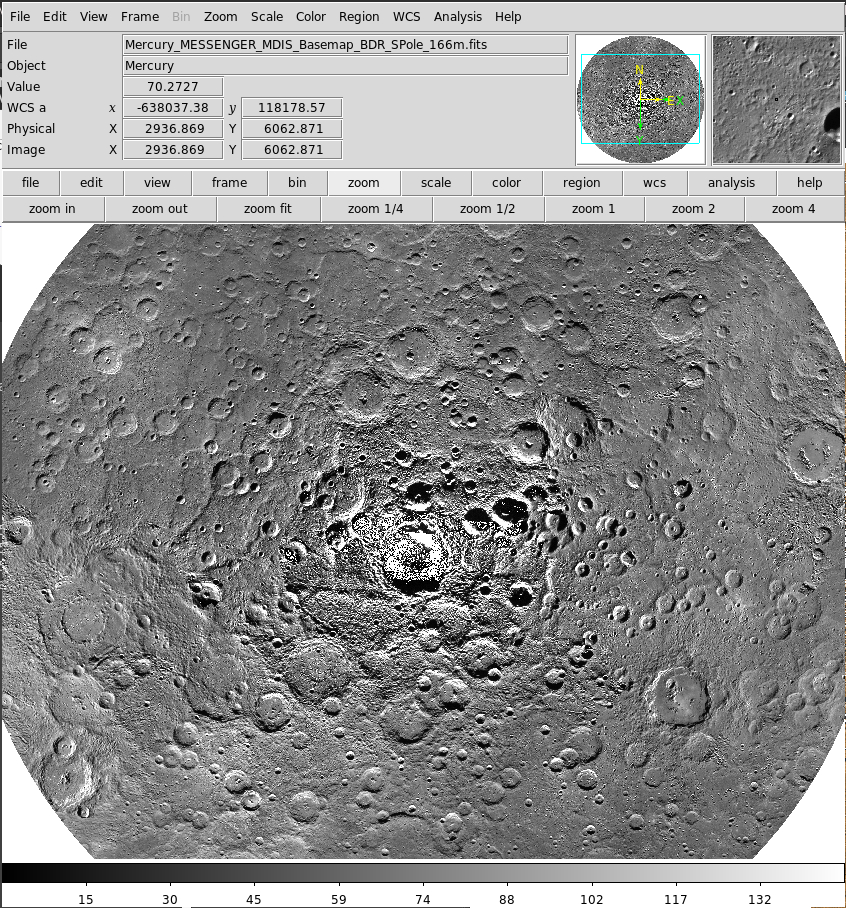
\includegraphics[height=17pc]{ess_marmo2} 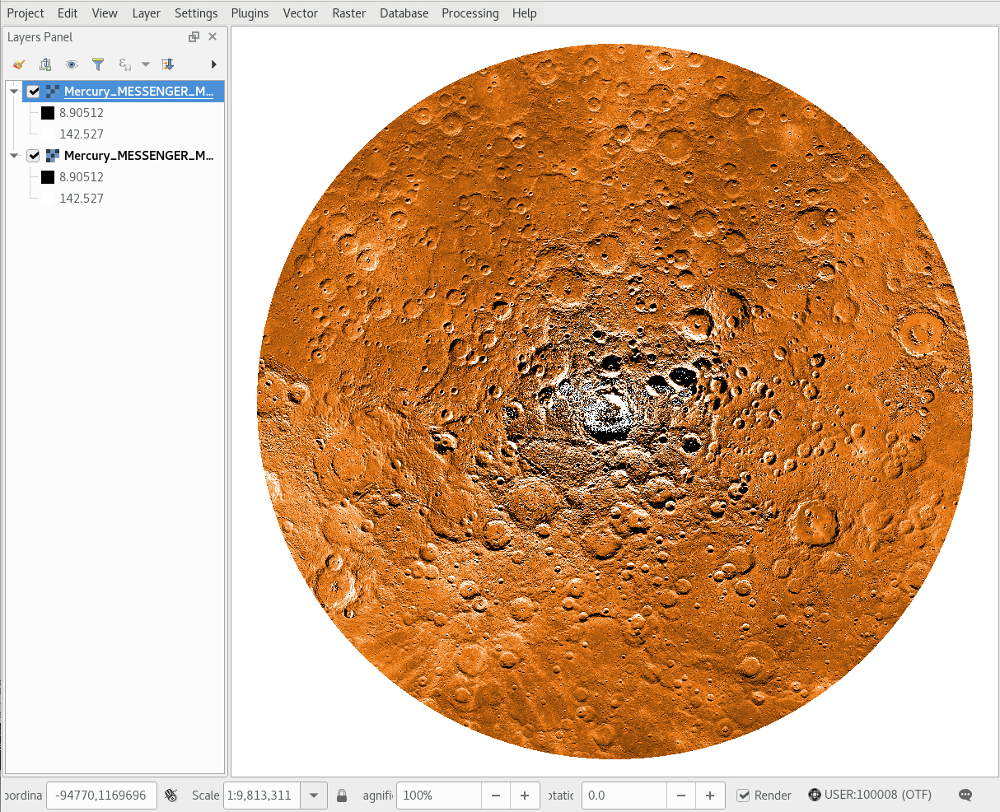
\includegraphics[height=17pc]{ess_marmo1}}
\caption{left: Mercury South Pole FITS image displayed in ds9;
right: GeoTIFF raster (displayed in yellow) and the virtual
header linked to the FITS raster (displayed in red); the two layers
are perfectly superposed.
Mercury image credits: MESSENGER Team, Arizona State University, Johns Hopkins Applied Physics
Laboratory, Carnegie Science}
\label{fig:ds9qgis}
\end{figure}

Assuming projected products are distributed in FITS format, a quick method to add GIS support for
FITS images is to use a GDAL-supported detached header.
GDAL Virtual Header files simply describe the internal structure of a FITS image, but
also the map projection and body size in a standardized "well known text"
(WKT) projection string.
As a result, the FITS raster loaded into QGIS thanks to its corresponding GDAL Virtual Header
is indistinguishable from the GeoTIFF layer (see figure \ref{fig:ds9qgis}, right side).

In order to load FITS files in GIS software, it is recommended to have
body radii and linear coordinates filled in.
Information about invalid values (NoData values) and minimum and maximum values are useful
to correctly display the image dynamics.

\subsubsection{OMEGA Spectra and Geometry Data}
As stressed above, having planetary data distributed in FITS at any processing level is
a way to avoid multiple conversions in the processing chain and to simplify reprocessing.
In planetary science spatial information is first provided for specific points over the detector
(the four corners of the detector, the center of each pixel, one or more pixel corners, etc.).
To support in FITS metadata such look-up table coordinate representation the \texttt{TAB}
algorithm has been defined in \citet{wcsspectral}.
In the \texttt{TAB} algorithm, coordinates are listed in a coordinate array, an indexing vector
can be used to address coordinate array elements.
Coordinates can then be sampled more or less coarsely depending on the behavior of the spatial
reconstruction.
Also, when the field is only partially covered by the planetary surface, coordinate array
dimensions can be significantly reduced. 
TAB projection is implemented in the Calabretta WCSLIB\footnote{http://www.atnf.csiro.au/people/mcalabre/WCS/wcslib/},
available in all major linux distribution.

As an example of non projected planetary data we have converted in FITS format some data
acquired by the imaging spectrometer OMEGA on-board of Mars Express.
OMEGA unprojected and uncalibrated data (level1b) are distributed by ESA-PSA and PDS archives.
Their structure is described in the OMEGA Experiment Archive 
Interface Control Document\footnote{ftp://psa.esac.esa.int/pub/mirror/MARS-EXPRESS/OMEGA/MEX-M-OMEGA-2-EDR-FLIGHT-V1.0/DOCUMENT/EAICD\_OMEGA.PDF}.
\begin{figure}[ht!]
\centerline{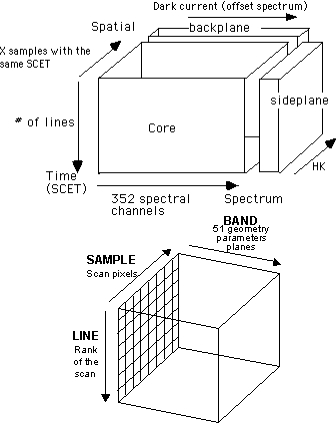
\includegraphics[height=17pc]{ess_marmo4}\hspace{2pc}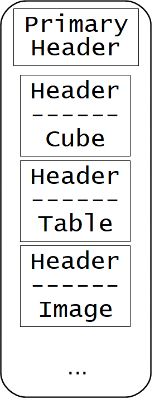
\includegraphics[height=17pc]{ess_marmo3}\hspace{2pc}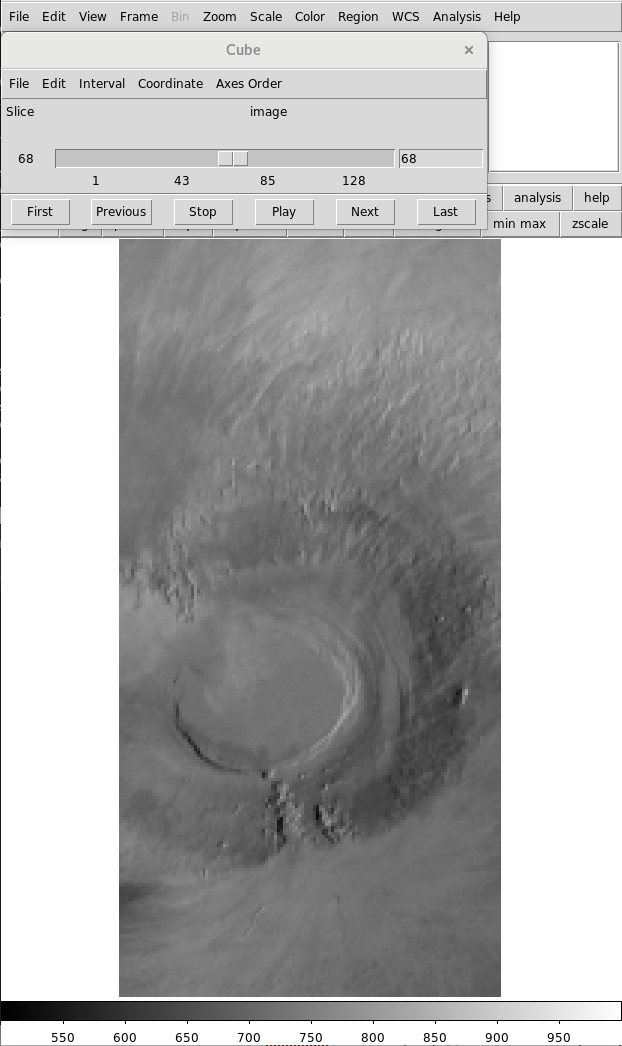
\includegraphics[height=17pc]{ess_marmo5}}
\caption{left: OMEGA data structure (from OMEGA EAICD), science data and geometry description are
distributed in different files; center: FITS Multi Digital Object scheme; as an example, we stored
the spectral data in the first cube extension, the coordinate look-up table in the second
extension, and other geometry parameters (incidence and emission angle, etc.) as images in the
following extensions; right: BSQ cube visualization with ds9.}
\label{fig:omegascheme}
\end{figure}

OMEGA rasters are equally sampled all over the field: we use them to exemplify
TAB description without indexing.
In addition, as geometrical description depends on the observation filter, this allows us to
distribute a file for each filter, containing science and geometry data.
The spectral cubes have been converted from Band Interleaved per Line (BIL) to Band Sequential
(BSQ) in order to make them easily understandable when visualized using standard FITS viewer
(as ds9 in figure \ref{fig:omegascheme})\footnote{The output result can be downloaded at the address https://github.com/cmarmo/convertofits/releases/download/v1.0-beta/orb0413\_1.IR1.fits.gz together with the python script used for conversion https://github.com/cmarmo/convertofits/blob/master/omega2fits.py}.

The \texttt{wcsware} tool (available in the \texttt{wcslib-utils} package in Fedora
distribution, in the \texttt{wcslib-tools} in Debian) had been run on the output file,
validating the WCS structure and checking the ability to convert to (\texttt{wcsware -w})
and from (\texttt{wcsware -x}) pixel and planetary surface coordinates.

\subsubsection{Akatsuki Imaging Data}
The Venus Climate Orbiter Akatsuki\footnote{http://akatsuki.isas.jaxa.jp/en/} is a JAXA
spacecraft dedicated to the study of the Venus atmosphere.
Akatsuki imaging data are already distributed in FITS format.
Geometry information is distributed in two different cubes of data, containing respectively 
values at the center of the pixel and at the lower left corner of the pixel.
Tabular coordinate representation allows us to gather geometry in one table together with
the described raster.
In addition to that, in Akatsuki images Venus is sometime far from completely filling the field:
tabular representation avoids to store unnecessary data. 
In that case, coordinate indexes are necessary to identify which pixels contains the spatial
information\footnote{The output result can be downloaded at the address https://github.com/cmarmo/convertofits/releases/download/v1.0-beta/ir1\_20160415\_070351\_097\_l2b\_v10\_out.fit.gz together with the python script used for conversion https://github.com/cmarmo/convertofits/blob/master/akatsukil2b.py}.

Again, we used \texttt{wcsware} to validate the WCS structure and to test pixel to world /
world to pixel coordinate conversion.
Even though TAB projection is not fully implemented in FITS visualization tools, this representation
has the advantage to store the detector geometrical information together with physical
quantities measured by the detector itself in a standardized way.

\section{Interoperable Software Developments}
\label{sec:softdev}
VO-QGIS-plugin\footnote{https://github.com/epn-vespa/VO\_QGIS\_plugin}

MATISSE\footnote{http://tools.asdc.asi.it/matisse.jsp} \citep{ZINZI2016}

Aladin\footnote{http://aladin.u-strasbg.fr/}

\section{Discussion and Perspectives}
\label{sec:disc}
FITS discussion in astronomy\citep{THOMAS2015133} 
let's astronomy learn from planetary sciences too: accent must be put on interoperability
.... blabla
Planetary surface is lacking open and general software for massive processing and can benefit
of astronomy experience. In addition to that WCS projection scheme is simpler than the
historical one used in planetary applications. 
Archiving flexibility and data model are today approached by PDS4 and EPN-TAP efforts.
Reducing custom data format conversions during the processing chain but
allowing easy conversion for final products following the needed application.

%%% End of body of article

%%%%%%%%%%%%%%%%%%%%%%%%%%%%%%%%
%% Optional Appendix goes here
%
% \appendix resets counters and redefines section heads
% but doesn't print anything.
% After typing \appendix
%
%\section{Here Is Appendix Title}
% will show
% A: Here Is Appendix Title
%
%\appendix
%\section{Here Is Appendix Title}
%This is an Appendix section.

%\begin{linenomath*}
%\begin{equation}asdf\end{equation}
%\end{linenomath*}

%%%%%%%%%%%%%%%%%%%%%%%%%%%%%%%%%%%%%%%%%%%%%%%%%%%%%%%%%%%%%%%%
%
% Optional Glossary, Notation or Acronym section goes here:
%
%%%%%%%%%%%%%%
% Glossary is only allowed in Reviews of Geophysics
%\begin{glossary}
%\term{Term}
% Term Definition here
%\term{Term}
% Term Definition here
%\term{Term}
% Term Definition here
%\end{glossary}

%
%%%%%%%%%%%%%%
% Acronyms
% \begin{acronyms}
% \acro{Acronym}
% Definition here
% \acro{EMOS}
% Ensemble model output statistics 
% \acro{ECMWF}
% Centre for Medium-Range Weather Forecasts
% \end{acronyms}

%
%%%%%%%%%%%%%%
% Notation 
% \begin{notation}
% \notation{$a+b$} Notation Definition here
% \notation{$e=mc^2$} 
% Equation in German-born physicist Albert Einstein's theory of special
%relativity that showed that the increased relativistic mass ($m$) of a
%body comes from the energy of motion of the body—that is, its kinetic
%energy ($E$)—divided by the speed of light squared ($c^2$).
% \end{notation}

%%%%%%%%%%%%%%%%%%%%%%%%%%%%%%%%%%%%%%%%%%%%%%%%%%%%%%%%%%%%%%%%
%
%  ACKNOWLEDGMENTS

\acknowledgments
This work benefits from support of VESPA/Europlanet.
The Europlanet 2020 Research Infrastructure is funded by the European Union
under the Horizon 2020 research and innovation program, grant agreement N.654208.
C. Marmo would like to thanks Mark Calabretta from Australia Telescope National Facility
for his WCSLIB library, and David Berry from Joint Astronomy Center, Hilo, for useful
discussions about TAB projection in FITS.

%%  REFERENCE LIST AND TEXT CITATIONS
%
% Either type in your references using
%
% \begin{thebibliography}{}
% \bibitem{}
% Text
% \end{thebibliography}
%
% Or, to use BibTeX:
%
% Follow these steps
%
% 1. Type in \bibliography{<name of your .bib file>} 
%    Run LaTeX on your LaTeX file.
%
% 2. Run BiBTeX on your LaTeX file.
%
% 3. Open the new .bbl file containing the reference list and
%   copy all the contents into your LaTeX file here.
%
% 4. Run LaTeX on your new file which will produce the citations.
%

\bibliography{ess_marmo}

% AGU does not want a .bib or a .bbl file. Please copy in the contents of your .bbl file here.


%\begin{thebibliography}{}


% % \bibitem[{\textit{Bell and Munoz}}(2008)]{Boug10} Bell, A.~H., and
% % Munoz, D.~P.  (2008). Activity in the superior colliculus reflects
% % dynamic interactions between voluntary and involuntary influences on
% % orienting behaviour. \textit{Eur. J. Neurosci.} 28, 1654--1660.

% % \bibitem[{\textit{Corbetta et~al.}}(1991)]{Buiz07} Corbetta, M.,
% % Miezin, F.~M., Dobmeyer, S., Shulman, G.~L., and Petersen, S.~E.
% % (1991). Selective and divided attention during visual discriminations
% % of shape, color, and speed: functional anatomy by positron emission
% % tomography. \textit{J.~Neurosci.} 11, 2383--2402.

% % \bibitem[{\textit{Borra et~al.}}(2014)]{Buiz98} Borra, E., Gerbella,
% % M., Rozzi, S., Tonelli, S., and Luppino, G.  (2014). Projections to
% % the superior colliculus from inferior parietal, ventral premotor, and
% % ventrolateral prefrontal areas involved in controlling goal-directed
% % hand actions in the macaque. \textit{Cereb. Cortex} 24, 1054--1065.

% % \bibitem[{\textit{Dorris et~al.}}(1997)]{Fra10}
% %  Dorris, M.~C.,
% % Par\'{e}, M., and Munoz, D.~P.  (1997). Neuronal activity in monkey
% % superior colliculus related to the initiation of saccadic eye
% % movements. \textit{J.~Neurosci.} 17, 8566--8579.

% % \bibitem[{\textit{Elsabbagh et~al.}}(2009)]{Ghel00} 
% % Elsabbagh, M.,
% % Volein, A., Holmboe, K., Tucker, L., Csibra, G., Baron-Cohen, S.,
% % et~al.  (2009). Visual orienting in the early broader autism
% % phenotype: disengagement. \textit{J.~Child Psychol. Psychiatry} 50,
% % 637--642.

% % \bibitem[{\textit{Fortin et~al.}}(1999)]{Gneit05} Fortin, S., Chabli,
% % A., Dumont, I., Shumikhina, S., Itaya, S.~K., and Molotchnikoff, S.
% % (1999). Maturation of visual receptive field properties in the rat
% % superior colliculus. \textit{bibain Res. Dev. Brain Res.} 1112,
% % 55--64.

% % \bibitem[{\textit{Felsen and Mainen}}(2008)]{Gneit07b} Felsen, G., and
% % Mainen, Z.~F.  (2008). Neural substrates of sensory-guided locomotor
% % decisions in the rat superior colliculus. \textit{Neuron} 60,
% % 137--148.

% % \bibitem[{\textit{Gattass and Desimone}}(1996)]{Haid14} Gattass, R.,
% % and Desimone, R.  (1996). Responses of cells in the superior
% % colliculus during performance of a spatial attention task in the
% % macaque. \textit{Rev. Bras. Biol.} 56, 257--279.

% % \bibitem[{\textit{Goldberg and Wurtz}}(1972)]{Hami00} Goldberg, M.~E.,
% % and Wurtz, R.~H.  (1972). Activity of superior colliculus in behaving
% % monkey. II. Effect of attention on neuronal responses.
% % \textit{J.~Neurophysiol.} 35, \hbox{560--574}.

% % \bibitem[{\textit{Krauzlis}}(2003)]{Kendall} Krauzlis, R.~J.  (2003).
% % Neuronal activity in the rostral superior colliculus related to the
% % initiation of pursuit and saccadic eye movements.
% % \textit{J.~Neurosci.} 23, 4333--4344.

% % \bibitem[{\textit{Heesy}}(2009)]{Leit74} 
% % Heesy, C.~P.  (2009). Seeing
% % in stereo: the ecology and evolution of primate binocular vision and
% % stereopsis. \textit{Evol. Anthropol.} 18, 21--35.

% % \bibitem[{\textit{Hilbig et~al.}}(2000)]{Mann45} Hilbig, H., Bidmon,
% % H.~J., Ettrich, P., and M\"{u}ller, A.  (2000). Projection neurons in
% % the superficial layers of the superior colliculus in the rat: a
% % topographic and quantitative morphometric analysis.
% % \textit{Neuroscience} 96, 109--119.

% % \bibitem[{\textit{Ignashchenkova et~al.}}(2004)]{Math76}
% % Ignashchenkova, A., Dicke, P.~W., Haarmeier, T., and Their, P.
% % (2004). Neuron-specific contribution of the superior colliculus to
% % overt and covert shifts of attention. \textit{Nat. Neurosci.} 7,
% % 56--64.

% \bibitem[{\textit{Krauzlis et~al.}}(2013)]{Palm00} Krauzlis, R.~J.,
% Lovejoy, L.~P., and Z\'{e}non, A.  (2013). Superior colliculus and
% visual spatial attention. \textit{Annu. Rev. Neurosci.} 36, 165--182.

% \bibitem[{\textit{Kustov and Robinson}}(1996)]{Papp09} Kustov, A.~A.,
% and Robinson, D.~L.  (1996). Shared neural control of attentional
% shifts and eye movements. \textit{Nature} 384, 74--77.

% \bibitem[{\textit{Landry and Bryson}}(2004)]{Park08} Landry, R., and
% Bryson, S.~E.  (2004). Impaired disengagement of attention in young
% children with autism. \textit{J.~Child Psychol. Psychiatry} 45,
% 1115--1122.

% \bibitem[{\textit{Kobayashi et~al.}}(2003)]{R2013} Kobayashi, T.,
% Tran, A.~H., Nishijo, H., Ono, T., and Matsumoto, G.  (2003).
% Contribution of hippocampal place cell activity to learning and
% formation of goal-directed navigation in rats. \textit{Neuroscience}
% 117, 1025--1035.

% \bibitem[{\textit{McHaffie et~al.}}(2005)]{Raft05} McHaffie, J.~G.,
% Stanford, T.~R., Stein, B.~E., Coizet, V., and Redgrave, P.  (2005).
% Subcortical loops through the basal ganglia. \textit{Trends Neurosci.}
% 28, 401--407.

% \bibitem[{\textit{McPeek and Keller}}(2004)]{Rich13} McPeek, R.~M.,
% and Keller, E.~L.  (2004). Deficits in saccade target selection after
% inactivation of superior colliculus. \textit{Nat. Neurosci.} 7,
% 757--763.

% \bibitem[{\textit{M\"{u}ller et~al.}}(2005)]{Scheu14} M\"{u}ller,
% J.~R., Philiastides, M.~G., and Newsome, W.~T.  (2005).
% Microstimulation of the superior colliculus focuses attention without
% moving the eyes. \textit{Proc. Natl. Acad. Sci. U.S.A.} 102, 524--529.

% \bibitem[{\textit{Munoz and Istvan}}(1998)]{ScheueBue13} Munoz, D.~P.,
% and Istvan, P.~J.  (1998). Lateral inhibitory interactions in
% the intermediate layers of the monkey superior colliculus.
% \textit{J.~Neurophysiol.} 79, 1193--1209.

%\end{thebibliography}

%%%%%%%%%%%%%%%%%%%%%%%%%%%%%%%%%%%%%%%%%
% Track Changes:
% To add words, \added{<word added>}
% To delete words, \deleted{<word deleted>}
% To replace words, \replace{<word to be replaced>}{<replacement word>}

% At the end of the document, use \listofchanges, which will list the
% changes and the page and line number where the change was made.

% When final version, \listofchanges will not produce anything,
% \added{} word will be printed, \deleted{} will take away the word,
% \replaced{}{} will print only the 2nd argument.

%%%
\listofchanges
%%%

\end{document}

%%%%%%%%%%%%%%%%%%%%%%%%%%%%%%%%%%%%%
%% Supporting Information
%% (Optional) See AGUSuppInfoSamp.tex/pdf for requirements 
%% for Supporting Information.
%%%%%%%%%%%%%%%%%%%%%%%%%%%%%%%%%%%%%


%%%%%%%%%%%%%%%%%%%%%%%%%%%%%%%%%%%%%%%%%%%%%%%%%%%%%%%%%%%%%%%

More Information and Advice:

%% ------------------------------------------------------------------------ %%
%
%  SECTION HEADS
%
%% ------------------------------------------------------------------------ %%

% Capitalize the first letter of each word (except for
% prepositions, conjunctions, and articles that are
% three or fewer letters).

% AGU follows standard outline style; therefore, there cannot be a section 1 without
% a section 2, or a section 2.3.1 without a section 2.3.2.
% Please make sure your section numbers are balanced.
% ---------------
% Level 1 head
%
% Use the \section{} command to identify level 1 heads;
% type the appropriate head wording between the curly
% brackets, as shown below.
%
%An example:
%\section{Level 1 Head: Introduction}
%
% ---------------
% Level 2 head
%
% Use the \subsection{} command to identify level 2 heads.
%An example:
%\subsection{Level 2 Head}
%
% ---------------
% Level 3 head
%
% Use the \subsubsection{} command to identify level 3 heads
%An example:
%\subsubsection{Level 3 Head}
%
%---------------
% Level 4 head
%
% Use the \subsubsubsection{} command to identify level 3 heads
% An example:
%\subsubsubsection{Level 4 Head} An example.
%
%% ------------------------------------------------------------------------ %%
%
%  IN-TEXT LISTS
%
%% ------------------------------------------------------------------------ %%
%
% Do not use bulleted lists; enumerated lists are okay.
% \begin{enumerate}
% \item
% \item
% \item
% \end{enumerate}
%
%% ------------------------------------------------------------------------ %%
%
%  EQUATIONS
%
%% ------------------------------------------------------------------------ %%

% Single-line equations are centered.
% Equation arrays will appear left-aligned.

Math coded inside display math mode \[ ...\]
 will not be numbered, e.g.,:
 \[ x^2=y^2 + z^2\]

 Math coded inside \begin{equation} and \end{equation} will
 be automatically numbered, e.g.,:
 \begin{equation}
 x^2=y^2 + z^2
 \end{equation}


% To create multiline equations, use the
% \begin{eqnarray} and \end{eqnarray} environment
% as demonstrated below.
\begin{eqnarray}
  x_{1} & = & (x - x_{0}) \cos \Theta \nonumber \\
        && + (y - y_{0}) \sin \Theta  \nonumber \\
  y_{1} & = & -(x - x_{0}) \sin \Theta \nonumber \\
        && + (y - y_{0}) \cos \Theta.
\end{eqnarray}

%If you don't want an equation number, use the star form:
%\begin{eqnarray*}...\end{eqnarray*}

% Break each line at a sign of operation
% (+, -, etc.) if possible, with the sign of operation
% on the new line.

% Indent second and subsequent lines to align with
% the first character following the equal sign on the
% first line.

% Use an \hspace{} command to insert horizontal space
% into your equation if necessary. Place an appropriate
% unit of measure between the curly braces, e.g.
% \hspace{1in}; you may have to experiment to achieve
% the correct amount of space.


%% ------------------------------------------------------------------------ %%
%
%  EQUATION NUMBERING: COUNTER
%
%% ------------------------------------------------------------------------ %%

% You may change equation numbering by resetting
% the equation counter or by explicitly numbering
% an equation.

% To explicitly number an equation, type \eqnum{}
% (with the desired number between the brackets)
% after the \begin{equation} or \begin{eqnarray}
% command.  The \eqnum{} command will affect only
% the equation it appears with; LaTeX will number
% any equations appearing later in the manuscript
% according to the equation counter.
%

% If you have a multiline equation that needs only
% one equation number, use a \nonumber command in
% front of the double backslashes (\\) as shown in
% the multiline equation above.

% If you are using line numbers, remember to surround
% equations with \begin{linenomath*}...\end{linenomath*}

%  To add line numbers to lines in equations:
%  \begin{linenomath*}
%  \begin{equation}
%  \end{equation}
%  \end{linenomath*}
